\documentclass{article}
\usepackage{graphicx} % Required for inserting images
\usepackage{amsmath}
\usepackage{amssymb}
\title{Analysing Overfitting in Deep Neural Networks}
\author{Divij Khaitan}
\date{\today}

\begin{document}

    \maketitle

    \section*{Experiment}
        The goal of this experiment was to try to see if there was a discernible pattern in the activations of neurons with respect to the respective weights. \\
        
        Given a neural network, the I approximated a Bernoulli probability distribution over the 'significant' activations of neurons of the $n-1$th layer and the weights in the final layer. A neuron activation was deemed to be significant if it had a 'large' absolute value relative to the absolute value of the sum across it's row or it's column. A large activation relative to a row signifies that the neuron-weight combination is significant to the row which corresponds to a class, while a large activation relative to a a column signifies that the class is important to the neuron in the previous layer. It is worth noting that this may not capture much information because it is entirely determined by the column of the weight matrix, \\

    \section*{Methodology}
        The final layer of the neural network operates as follows. Given an activation vector $x \in \mathbb{R}^{4096 \times 1}$ and a weight matrix $W \in \in \mathbb{R}^{1000 \times 4096}$ \\
        \[
            \begin{bmatrix}
                w_{1,1} & \dots & w_{1,4096} \\
                \vdots & \ddots & \vdots \\
                w_{1000, 1} & \cdots & w_{1000, 4096} \\
            \end{bmatrix}
            \begin{bmatrix}
                x_1 \\
                \vdots \\
                x_{4096} \\
            \end{bmatrix}
            = 
            \begin{bmatrix}
                w_{1,1}x_1 + w_{1, 2}x_2 + \dots + w_{1, 4096}x_{4096} \\
                \vdots \\
                w_{1000,1}x_1 + w_{1000, 2}x_2 + \dots + w_{1000, 4096}x_{4096}
            \end{bmatrix}
        \]
        This would not allow us to study the individual activation-weight pairs, because they would all be summed up. A vector operation that computes the sum over the rows of a matrix is postmultiplication by the all 1s vector, so by factoring out this vector we can get the required information. Factoring out the all 1s vector from the neurons in the penultimate layer, we get an diagonal matrix with the neurons activations as entries \\
        \[
            \begin{bmatrix}
                w_{1,1} & \dots & w_{1,4096} \\
                \vdots & \ddots & \vdots \\
                w_{1000, 1} & \cdots & w_{1000, 4096} \\
            \end{bmatrix}
            \begin{bmatrix}
                x_1  & \dots & 0 \\
                \vdots & \ddots & \vdots \\
                0 & \dots & x_{4096} \\
            \end{bmatrix}
            = 
            \begin{bmatrix}
                w_{1,1}x_1  & \dots & w_{1,4096}x_1 \\
                \vdots & \ddots & \vdots \\
                w_{1000, 1}x_{4096} & \dots & w_{1000, 4096}x_{4096} \\
            \end{bmatrix}
        \]
        
        \section*{Results}
            The result of fitting a binomial distribution to the data is a $1000 \times 4096$ matrix of vectors in the ball of length 1 in the supremum norm. This can also be interpreted as a probability distribution. I have looked at the eculidean distance between the vectors, as well as the KL divergences between the binomial distributions defined by the vector. The results for both are presented below. It is worth noting that when looking at significance relative to the rest of the row, there were several entries where the activation proportion was 1. The KL divergence is not defined relative to a constant, the array was clipped at ($10^{-7}, 1 - (10^{-7})$), where values outside the range are appropriately mapped to the relevant bound.
            \begin{figure}[ht]
                \centering
                \begin{minipage}{\textwidth}
                    \centering
                    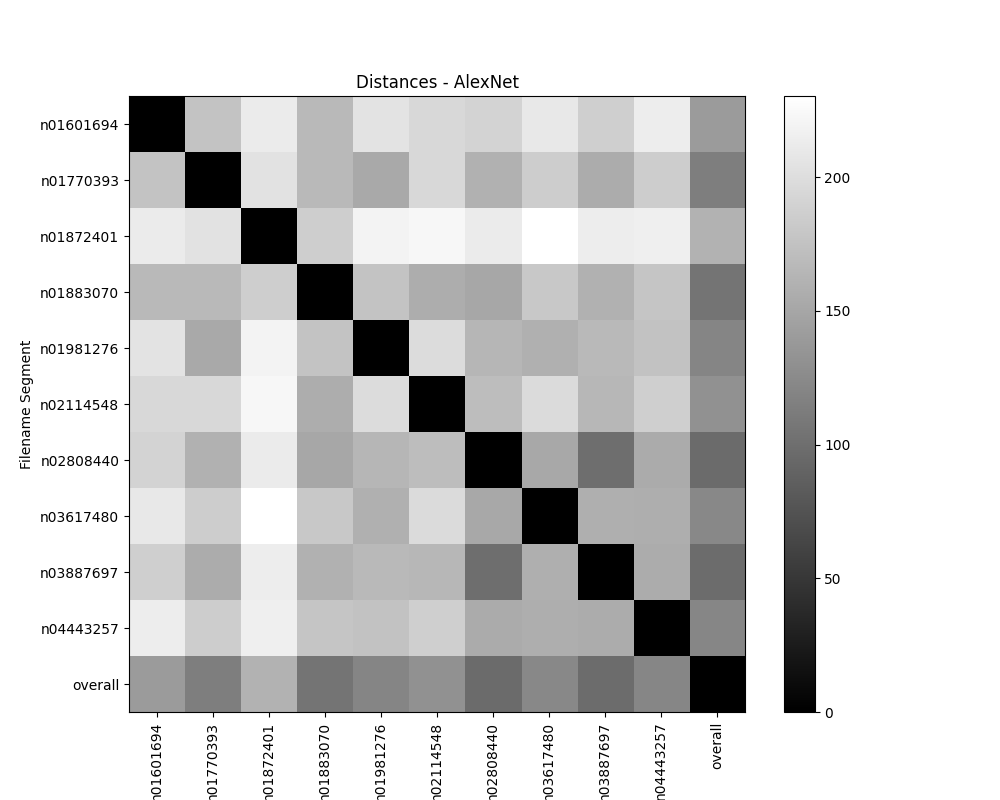
\includegraphics[width=\textwidth]{AlexNet_d_matrix.png} % first image
                    
                \end{minipage}\hfill
                \begin{minipage}{\textwidth}
                    \centering
                    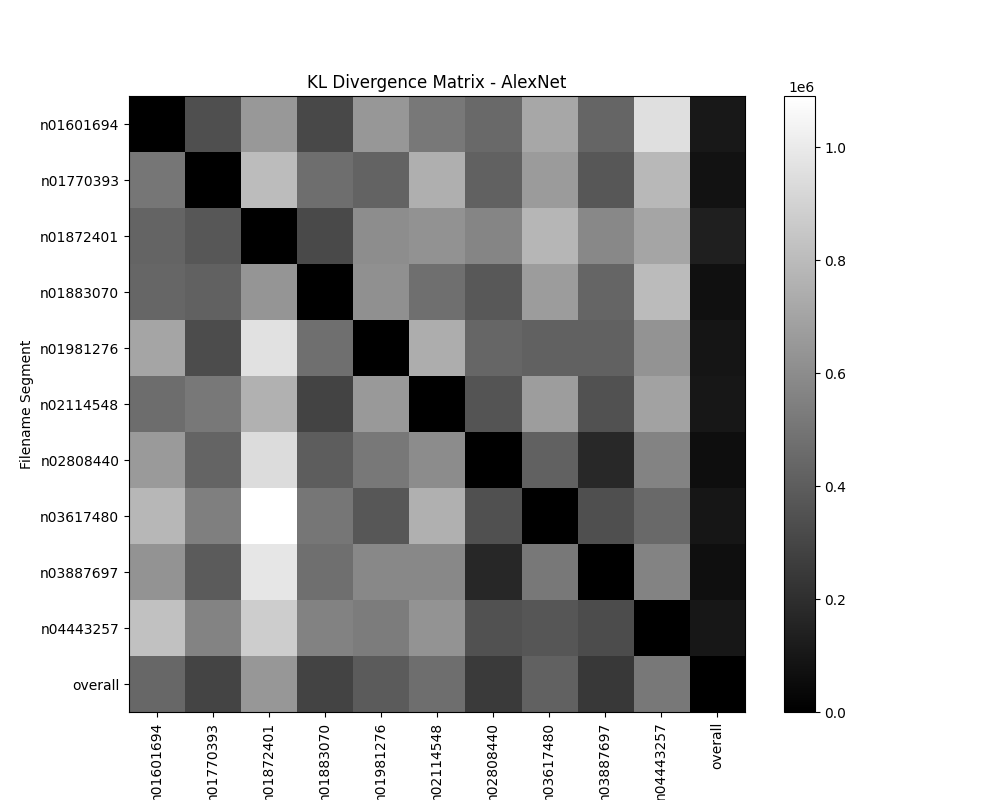
\includegraphics[width=\textwidth]{AlexNet_kl_matrix.png} % second image
                \end{minipage}
                \caption{Pairwise KL Divergences and Distances between the significance distributions for Alexnet. Notice the small scale for the KL Divergences}
                \label{fig1}
            \end{figure}
            \begin{figure}[ht]
                \centering
                \begin{minipage}{\textwidth}
                    \centering
                    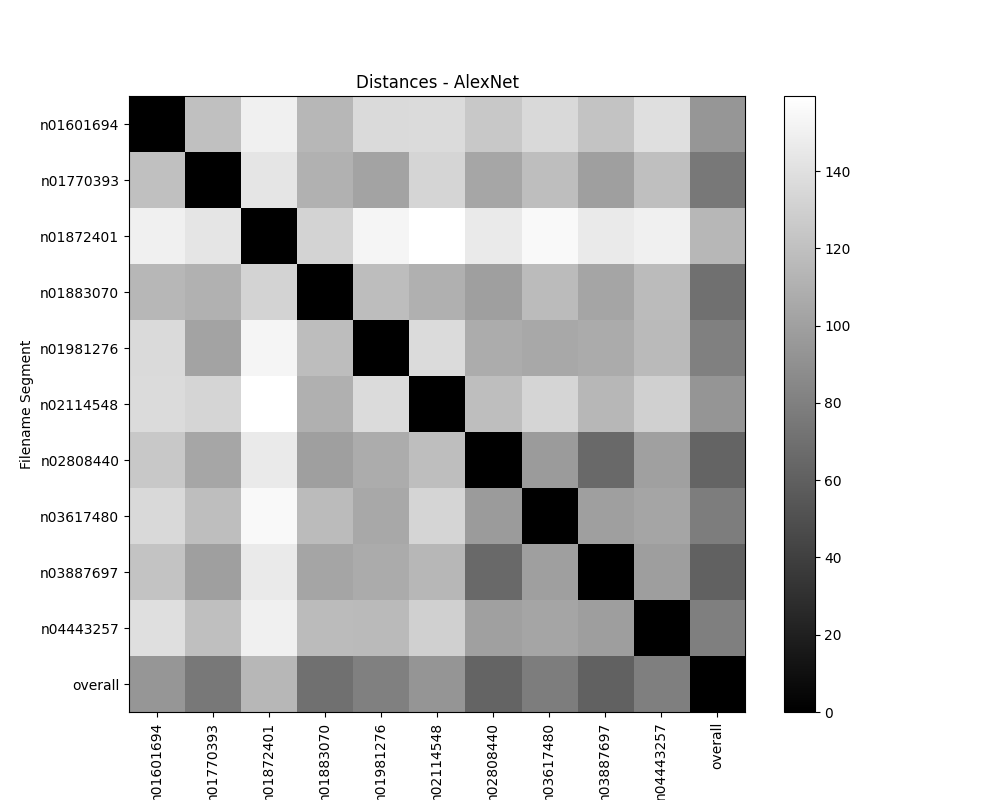
\includegraphics[width=\textwidth]{AlexNet_d_matrix_column.png} % first image
                    
                \end{minipage}\hfill
                \begin{minipage}{\textwidth}
                    \centering
                    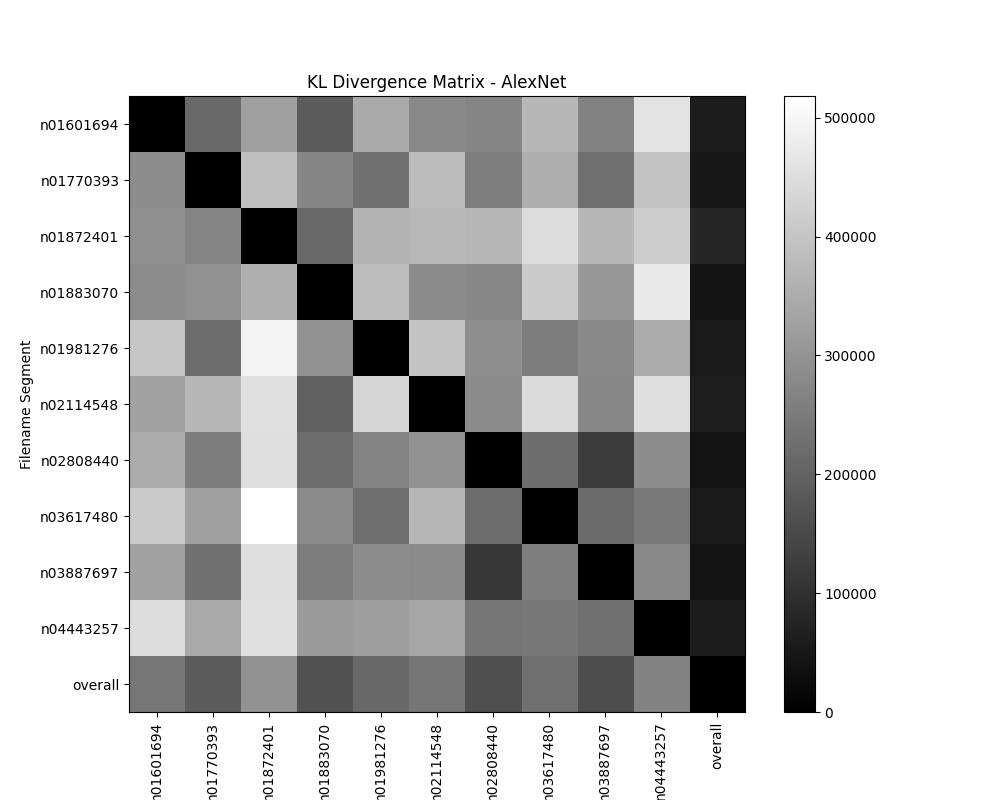
\includegraphics[width=\textwidth]{AlexNet_kl_matrix_column.png} % second image
                \end{minipage}
                \caption{Pairwise KL Divergences and Distances between the significance distributions for Alexnet. Notice the small scale for the KL Divergences}
                \label{fig1}
            \end{figure}
            
\end{document}